\expandafter\ifx\csname ifdraft\endcsname\relax
 \documentclass{jsarticle}
 \begin{document}
\fi
\section  {導入}
%銀河の速度からかみのけ座銀河団の質量出して、閑話休題したあとシミュレーションでビリアル定理確認
このレポートでは、自己重力系のビリアル定理についてまとめる。まずN質点系におけるビリアル定理について重力相互作用を考慮に入れた運動方程式から導かれることを確認する。そして自己重力系としての銀河団について考え、かみのけ座銀河団の質量を概算する。その後、実際に多体系でのシミュレーションを行いビリアル定理を確認する。また、その過程において銀河団や数値計算法についてのいくつかの説明を加える。
\section  {ビリアル定理}
\subsection{多体系の運動方程式}
多体系の運動方程式は以下のように書ける。
\begin{equation}
	m_i \frac{d^2x_i}{dt^2} = \sum_{i \neq j} f_{ij}
\end{equation}	
ここで$f_{ij}$は、$G$を重力定数として、
\begin{equation}
	f_{ij} = G m_i m_j \frac{x_j - x_i}{|x_j - x_i|^3}
\end{equation}	
この運動方程式は、二対問題、円制限三体問題などの特殊な三体問題、粒子数無限の極限における平衡解などでは解析的、近似的に解けるがほとんどの場合解けない。
しかし、数値計算を用いれば原理的には必ず解を求めることができる。原理的にはと付け加えたのは実際には計算資源は有限であり、銀河の星の数は$10^{11}$のオーダーであるにも関わらず
数値計算では高々$10^5$くらいの計算しかできない。
また、数値計算で解のみを求めても物理的な理解にはあまり繋がらない。
そこで、次の章での数値計算の理解を深めるために、この章ではまず無衝突ボルツマン方程式の空間的モーメントからビリアル定理を得る。
また、ビリアル定理の直接的な応用としてかみのけ座の質量推定を行う。

\subsection{無衝突ボルツマン方程式}
以下では、$\Phi$を重力ポテンシャル、$f(\evec{x}, \evec{v}, t)$を6次元位相空間での分布関数とする。
位相空間$\omega = (\evec{x}, \evec{v})$での流れの速度は、$\dot{\omega} = (\dot{\evec{x}}, \dot{\evec{v}})$で、
連続の式は、
\begin{equation}	
	\frac{\partial f}{\partial t} + \sum_i \frac{\partial (f(\dot{\omega_i}))}{\partial \omega_i} = 0
\end{equation}	
であり、ここから無衝突ボルツマン方程式を得る。
\begin{equation}	
	\label{bolzman}
	\frac{\partial f}{\partial t} + \evec{v}\cdot\nabla f - \nabla\Phi\cdot\frac{\partial f}{\partial \evec{v}}= 0
\end{equation}	
これは$f$のラグランジュ微分である。
\subsection {自己重力系のビリアル定理}
ボルツマン方程式の速度のモーメントからはジーンズ方程式が得られる。
0次の速度モーメントは、流体力学での連続の式、1次の速度モーメントはオイラー方程式、つまり運動方程式に対応する。ビリアル定理は、空間のモーメントから得られる。
ここでボルツマン方程式は無衝突の場合を指すこととする。

となる。これは自己重力系のビリアル定理である。

\section {N体シミュレーション}
\subsection {リープフロッグ法}
リープフロッグ法はN体シミュレーションで広く使われている二次の積分法である。
公式は
\begin {equation}
    v_{\frac{1}{2}} = v_0 + \frac{a_0}{2dt}\\
\end {equation}
\begin {equation}
    x_1 = x_0 +v_{\frac{1}{2}}dt 
\end {equation}
\begin {equation}
    v_1 = v_{\frac{1}{2}} + \frac{a_1dt}{2}
\end {equation}
となる。このアルゴリズムではまず半ステップ先の速度を計算し、この速度を使って位置更新する。これはシンプレクティック解法の一種であり、ルンゲクッタ法などよりも保存系の力学を解くことに優れている。
また、加速度が速度に依存しないことから重力計算によく用いられる。
\subsection {設定}
N体シミュレーションの流れは以下のようになる。
\subsubsection{パラメータ設定}
$\epsilon$:ソフトニングパラメーター (初期値 0.003125)\\
$dt$:時間積分のタイムステップ (初期値 2500)\\
$t_end$:シミュレーションの終了時刻 (初期値 5)\\
ここで、ソフトニングパラメーターとは距離の逆数を計算をする際に発散を防ぐために導入される系の大きさに対して微小な項である。

\subsubsection{初期分布設定} 
ここでは温度分布と粒子分布を指定する。
粒子分布を作成する際には初期速度分布も作成しなくてはならない。
今回は等温一様球を初期条件とする。
位置分布は指定された粒子数の分だけx,y,zを一様乱数で[-1,1]で作成し、その中で平方二乗和が1以下ののもを選ぶことで得る。単位球を採用し、粒子数は200とした。
初期速度分布は平均0、分散$\sigma$のガウス分布を用いるが、速度分散は与えられたビリアル比から計算する。ビリアル比$r_v=0.1$とした。
ビリアル比$r_v$は、$r_v = \frac{K}{|W|}$と定義される。
$K$は系の運動エネルギー、$W$はポテンシャルエネルギーの和である。
\begin{equation}
    \sigma = (\frac{2r_v|W|}{3M})^{\frac{1}{2}}
\end{equation}
から速度分散が計算される。
\subsubsection{相互重力計算}
ここでは、相互重力計算に直接法を用いる。つまり粒子iに対して、
\frac{d^2x}{dt^2} = \sum_{j i}
\subsection {結果}
シミュレーションの結果、図1のような結果が得られた。
ビリアル比ー時間のグラフに注目すると、初期設定では0.1だったビリアル比が、
2/3に漸近していることがわかる。これは自己重力系のビリアル定理を確認する。
また、シンプレクティック積分をしているので平衡状態でのエネルギー誤差は微小である。
\begin{figure}[b]
    \label{fig:result}
    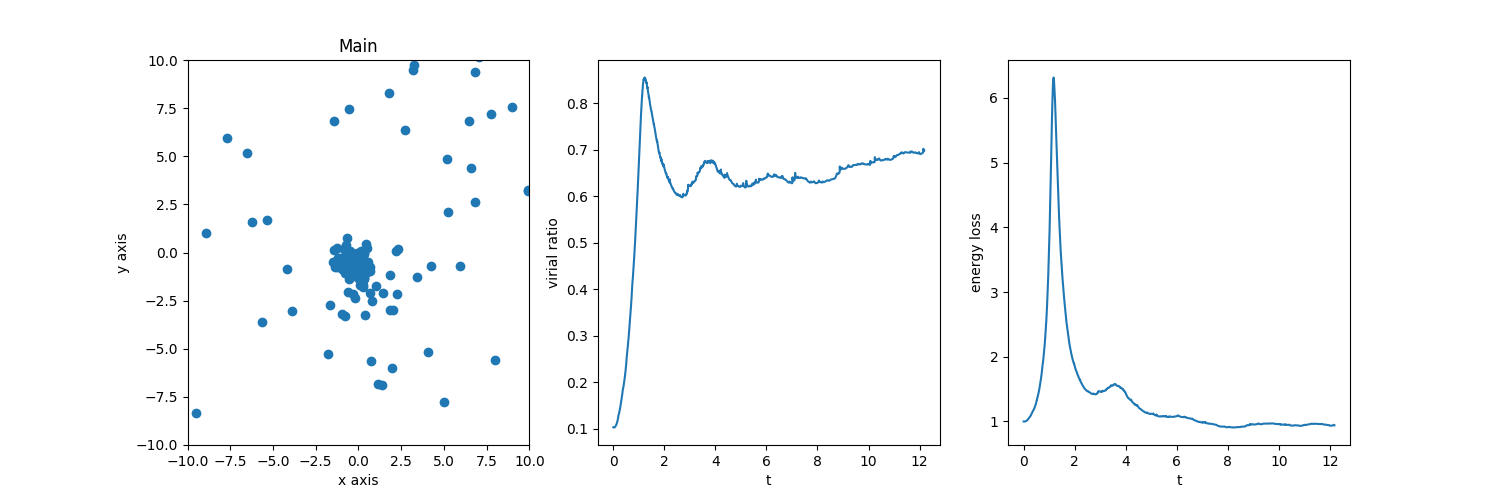
\includegraphics[width=\textwidth,natwidth=1000,natheight=642]{fig.png}
    \caption{x-y分布、ビリアル比ー時間、エネルギー誤差ー時間}
\end{figure}
\expandafter\ifx\csname ifdraft\endcsname\relax
  \end{document}
\fi
